
\subsection{Numeryczne wyznaczanie krzywych dyspresji}
Pierwszym przypadkiem numerycznego wyznaczania krzywych dyspersji, jest rozwiązanie równań Rayleigha-Lamba przedstawionych w poprzedniej sekcji. Zakładamy, że interesują nas tylko rozwiązania rzeczywiste, które pojawią się jeśli k przyjmie wartości rzeczywiste bądź urojone (w równaniach występuje tylko czynnik \(k^2\)).

Poniżej znajdują się równania Rayleigha-Lamba w postaci ułatwiającej proponowany sposób rozwiązania:

\begin{equation}
\frac{tan(qh)}{q}+\frac{4k^2ptan(ph)}{{q^2-k^2}^2}=0
\end{equation}

\begin{equation}
qtan(qh)+\frac{{(q^2-k^2)}^2tan(ph)}{2k^2p}=0.
\end{equation}

\vspace{5mm}

Rozwiązać równanie możemy według przedstawionego algorytmu.

\begin{enumerate}
  \item Wybierz iloczyn \((\omega h)_0\).
  \item Wybierz początkową estymatę prędkości fazowe \((c_p)_0\) (a pośrednio też \(k\)).
  \item Oblicz znak lewych stron równań R-L.
  \item Wybierz kolejną wartość prędkości fazowej \((c_p)_1 > (c_p)_0\) i policz znaki lewych stron jeszcze raz.
  \item Powtarzaj kroki 3 i 4 aż znaki się zmienią. Oznaczać to bedzie, że pierwiastek równania znajduje się pomiędzy ostatnio wybranymi prędkościami. Załóżmy, że jest to pomiędzy \( (c_p)_n \) i \( (c_p)_{n+1} \).
  \item Wykorzystaj jakiś algorytm iteraycjny do znalezienia pierwiastka \(c_p\) z odpowiednią dokładnością.
   \item Po znalezienu pierwiastka, kontynuuj wyszukiwnie kolejnych pierwiastków dla założonego \( (\omega h)_0 \), powtarzając kroki 2-6.
  \item Wybierz kolejną wartość \( \omega h \) i wykonaj dla niej kroki 2-7.
\end{enumerate}

\vspace{5mm}

W ten sposób łatwo wyznaczyć krzywe dyspersji, ale należy zaznaczyć, że równania dyspersyjne zostały obliczone analitycznie dla konkretnego przypadku struktury, jaką jest płyta. Metody numeryczne ograniczają się w tym przypadku do rozwiązania wyznaczonych równań. Możliwość ogólniejszego podejścia do badań numerycznych, dla szerokiego wachlarza struktur daje metoda elementów skończonych.

Metoda ta daje możliwości dokładnego przewidzenia odpowiedzi dynamicznych, dla złożonych układów mechanicznych. Jeśli założymy przypadek małych odkształceń, to problem można zapisać w postaci równania różniczkowego:

\begin{equation} \label{eq:MES1}
M\ddot u + Ku = f^{ext}
\end{equation}

gdzie
\begin{eqwhere}[2cm]
        \item[$M$] macierz mas układu
        \item[$K$] macierz sztywności układu 
        \item[$u$] przemieszczenia punktów układu
        \item[$f^{ext}$] wektor sił zewnętrznych
\end{eqwhere}

Sposobem wyznaczenia krzywych dyspersji z tak określonego układu, może być rozwiązanie równania tj. znalezienie pola przemieszczeń dla wszystkich węzłów w dyskretnych chwilach czasowych, a następnie obliczenie wielowymiarowego przekształcenia Fouriera otrzymanego sygnału.

Równanie można rozwiązać na przykład z wykorzystaniem centralnej formuły różnicowej dla \( \ddot u\):

\begin{equation}
\ddot x = \frac{u^{t+1} - 2u^t + u^{t-1}}{\Delta t^2}.
\end{equation}

Po podstawienu otrzymujemy zależność:

\begin{equation}
\frac{1}{\Delta t^2}M(u^{t-1}-2u^t+u^{t-1}) + Ku^t = f^t
\end{equation}

\begin{equation}
u^{t+1}=\Delta t^2 M^{-1}(f^t -Ku^t)+2u^t-u^{t-1}
\end{equation}

gdzie \( t \) oznacza obecną chwilę czasową, a \( t+1 \) chwilę kolejną.
Operacja odwracania macierzy mas jest kosztowna obliczeniowo. Można przyśpieszyć obliczenia przez zastosowanie skupionej macierzy mas (wyrazy niezerowe tylko na głownej diagonali).

Jeśli interesuje nas propagacja tylko w jednym kierunku, to dla obliczonego sygnału \( u[m, n] \) (m - liczba kroków czasowych \(\Delta t \) , n - liczba kroków geometrycznych \(\Delta x\) w kierunku x) przekształcenie Fouriera można obliczyć według wzoru:

\begin{equation} \label{eq:fourier_2d}
U[p, q] = \sum_{k=0}^{m-1} \sum_{l=0}^{n-1} u[k, l]e^{-i2\pi (-p \frac{k}{m} + q\frac{l}{n})}
\end{equation}

Mając dyskretną postać przekształcenia Fouriera można wykreślić krzywe dyspersji, wyznaczając dla każdej próbki wartość czętotliwości i liczby falowej. Można to zrobić wiedząc, że częstość zawiera się w przedziale \([0, \frac{1}{2\Delta t}2\pi]\), a liczba falowa \([0, \frac{1}{2\Delta x}2\pi]\). Przykładowe krzywe przedstawione są na rysunku \ref{fig:krzywe_dyspersji_tian1}.

\vspace{5mm}

\begin{figure}[h]
\centering
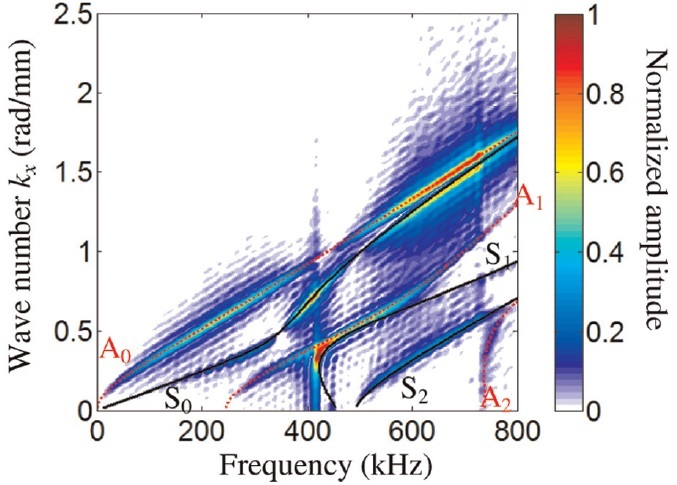
\includegraphics[width=10cm]{Zdjecia/2/dyspersja_tian1}
\caption{Krzywe dyspersji wyznaczone przy pomocy dwuwymiarowego DFT}
\label{fig:krzywe_dyspersji_tian1}
\end{figure}

Innym sposobem wyznaczania krzywych dyspersji z pomocą modelu MES, jest symulacja układu dla wymuszeń harmonicznych o ustalonych częstotliwościach, w których chcemu wyznaczyć krzywe. Jako przyład rozpatrzmy jednorodny pręt. Dla przypadku pręta wymuszanego na jednej płaszczyźnie przekroju, dane należy zebrać przed odbiciem fali od swobodnego końca pręta, tak aby sygnał propagował tylko w jednym kierunku. W liniach równoległych do osi, obliczamy pola prędkości przemieszczenia punktów. Może to być też pole przemieszczeń lub naprężeń, ale pole prędkości jest stosunkowo łatwe do wyznaczenia.
Znając już prędkości dla wszystkich punktów w jednej lini, w chwili t, możemy wyznaczyć widmo otrzymanego sygnału. Następnie z widma sygnału odczytujemy liczby falowe, dla których powstały widoczne piki. Pik dla największej liczby falowej dotyczy pierwszego modu, a każdy kolejny, z coraz mniejszymi liczbami falowymi, modów kolejnych.

Pole prędkości można wyznaczyć na podstawie różnycowych formuł centralnych \ref{eq:MES2} oraz \ref{eq:MES3}.

\begin{equation} \label{eq:MES2}
\dot u^{t+1} = \dot u^n + \frac{\Delta t}{2}(\ddot u^n + \ddot u^{n+1})
\end{equation}

\begin{equation} \label{eq:MES3}
u^{n+1} = u^n + \Delta t(\dot u^n + \frac{\Delta t}{2}\ddot u^n)
\end{equation}

Załóżmy, że znamy pełne rozwiązanie w chwili t. Przemieszczenie w chwili t+1 możemy więc obliczyć z zależności \ref{eq:MES3}. Następnie podstawiamy wynik do równania \ref{eq:MES1} i obliczamy przyspeszenie w chwili t+1. Ostatecznie korzystając z formuły \ref{eq:MES2} możemy wyznaczyć prędkość w chwili t+1.

Przykładowe widmo, z którego możemy odczytać liczby falowe czterech modów znajduje się na rysnuku \ref{fig:widmo_wymuszenie1}. Jak widać nie wszystkie liczby falowe da się wykryć przy pomocy danych z jednej lini, więc niezbędne jest prowadzenie obliczeń dla kilku różnych linii.

\begin{figure}[h]
\centering
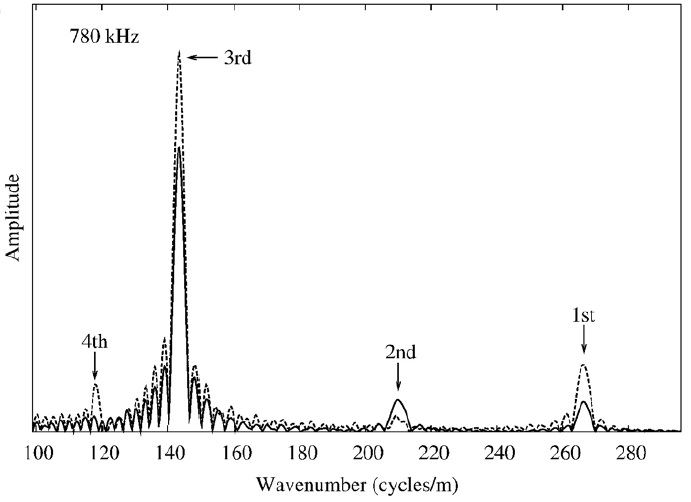
\includegraphics[width=10cm]{Zdjecia/2/widmo_wymuszenia_waskopasmowe}
\caption{Widmo sygnału prędkości na liniach równoległych do osi pręta}
\label{fig:widmo_wymuszenie1}
\end{figure}

Wadą tego sposobu jest konieczność prowadzenia obliczeń dla każdej częstotliwości, dla jakiej chcemy mieć punkty krzywych dyspersji. Jedne przebieg daję nam tylko jeden punkt na każdej krzywej. Fakt prowadzenia obliczeń tylko w liniach równoległych do osi pręta, ogranicza dodatkow obszar propagujących fal do fal podłużnych.

\vspace{3mm}

Sposobem zmniejszenia liczby symulacji jakie trzeba przeprowadzić jest symulacja z wymuszeniem szerokopasmowym. Pozwala to na uzyskanie informacji o krzywych dyspersji, dla częstotliwości zawierających się w wymuszającym sygnale. Pojawia się jednak kilka dodatkowych kroków jakie trzeba wykonać, aby uzyskać liczby falowe modów dla poszczególnych częstotliwości.

Aby uzyskać dane do wykreślenia krzywych dyspersji, należy obliczyć przestrzenny rozkład prędkości na liniach równoległych do osi dla wszystkich częstotliwości. W tym celu trzeba wykonać następujące czynności.

\begin{enumerate}
  \item Wyznaczyć odpowiedzi czasowe dla każdego punktu na interesującej nas lini równoległej do osi pręta.
  \item Obliczyć transformaty Fouriera tych sygnałów
  \item Z widma sygnału w każdym punkcie pobrać informacje o amplitudzie dla kolejnych częstotliwości. Na tej podstawie odtworzyć amplitudowy przebieg sygnału na całej lini dla każdej interesującej nas częstotliwości.
  \item Dla obliczonych w pkt. 3 przebiegów, obliczyć transformatę Fouriera i z wykresu odczytać wartości liczby falowej, dla wybranych częstotliwości.
\end{enumerate}

Rysunki \ref{fig:szer_odp_czasowe} oraz \ref{fig:szer_odp_przestrzenne} przedstawiają kolejne kroki postępowania, dla odpowiedzi na wymuszenie krokiem jednostkowym preta zbudowanego z 1601 węzłów na długości jednej lini. 

\begin{figure}[h]
\centering
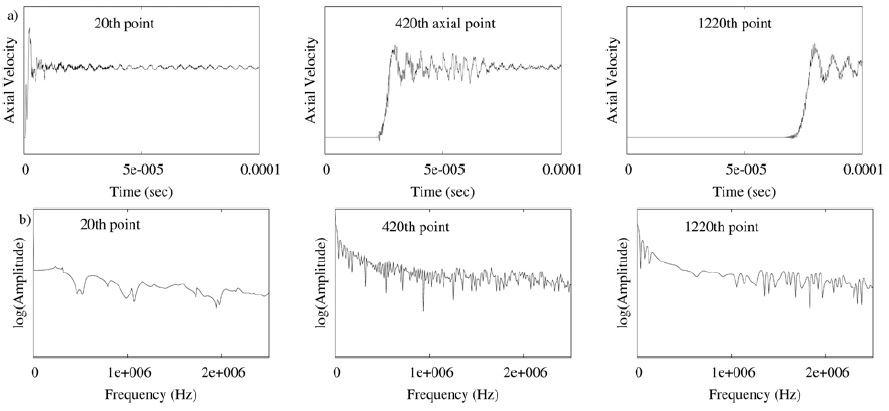
\includegraphics[width=12cm]{Zdjecia/2/widmo_wymuszenia_szerokopasmowe1}
\caption{a) Odpowiedzi na szerokopasmowe wymuszenie w wybranych punktach jednej lini b) Przekształcenia Fouriera odpowiedzi czasowych}
\label{fig:szer_odp_czasowe}
\end{figure}

\begin{figure}[h]
\centering
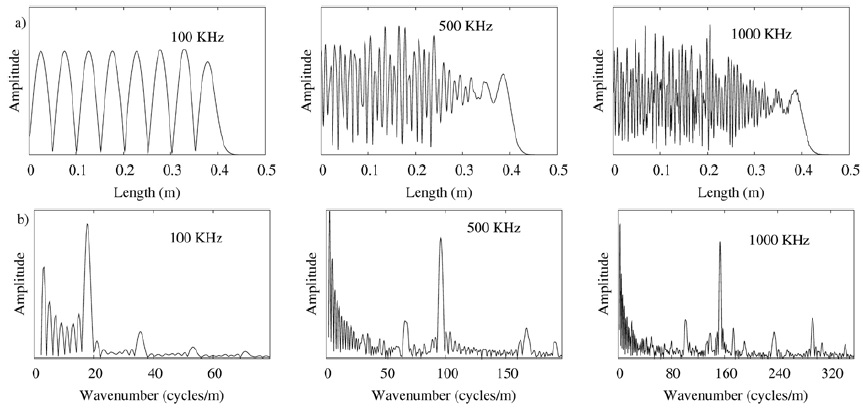
\includegraphics[width=12cm]{Zdjecia/2/widmo_wymuszenia_szerokopasmowe2}
\caption{a) Odtworzony sygnał apmlitudowy na długości pręta w jednej lini b) Przekształcenie Fouriera odtworzonych sygnałów}
\label{fig:szer_odp_przestrzenne}
\end{figure}

\vspace{3mm}

Ostatnia przedstawiona tutaj metoda skupia się, na rozwiązaniu zagadnienia własnego modelu wyznaczonego z pomocą MES. Tym razem zakładać będziemy wybraną liczbę falową i dla niej obliczać częstości poszczególnych modów. 
Po raz kolejny za przykład weźmy pręt. Pręt dzielimy na komórki, które będą się składać z kolejnych płaszczyzn, na których znajdują się węzły. Znając odległość płaszczyzn i wybierając liczbę falową, możemy okrelić przesunięcie fazowe fali pomiędzy płaszczyznami. Sytuacja przedstawiona jest na rysunku \ref{fig:komorki_preta}.


\begin{figure}[h]
\centering
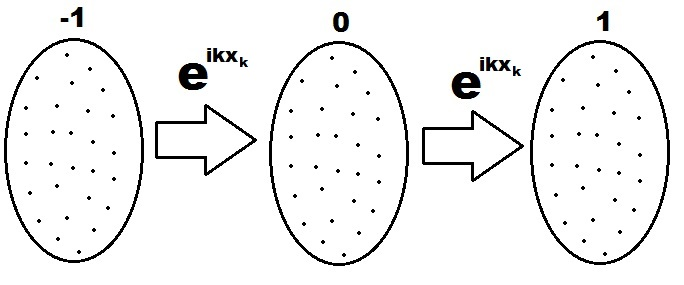
\includegraphics[width=10cm]{Zdjecia/2/metoda_numeryczna3}
\caption{Kolejne komórki pręta}
\label{fig:komorki_preta}
\end{figure}

W liniowych systemach do opisu popagacji fali wystarcza jedna komórka i siły wewnętrzne pochodzące od komórek sąsiednich. W przypadku braku sił zewnętrznych i przy założeniu skupionej macierzy mas, równanie układu można zapisać w postaci \ref{eq:MES4}. Rysunek \ref{fig:komorki_preta_sztywnosc} przedstawia sposób wyznaczania macierzy sztywności dla komórki środkowej, z uwzględnieniem zależności z komórkami sąsiednimi.

\begin{equation} \label{eq:MES4}
M_0\ddot x_0 + \sum_{p=-1}^1 K_p x_p = 0
\end{equation}

\begin{figure}[h]
\centering
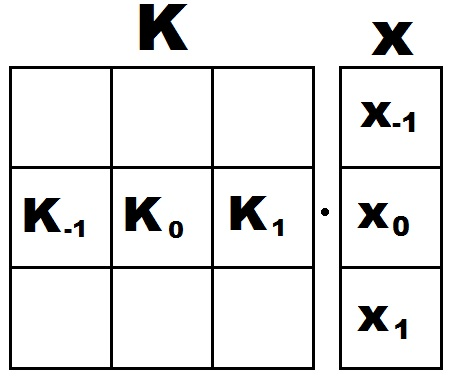
\includegraphics[width=8cm]{Zdjecia/2/metoda_numeryczna3_sztywnosc}
\caption{Wyznaczanie macierzy sztywności środkowej komórki z uwzględnieniem zależności z komórkami sąsiednimi}
\label{fig:komorki_preta_sztywnosc}
\end{figure}

Uwzględniając wszystkie informacje równanie układu można zapisać jako \ref{eq:MES5}. Podstawiając dodatkowo zależności \( \ddot x = x \omega^2 \), \( M_{sys} = M_0 \) oraz \( K_{sys} = K_{-1} e^{-ikx_k} + K_0 + K_1 e^{ikx_k} \) otrzymujemy równanie \ref{eq:MES6}.

\begin{equation} \label{eq:MES5}
M_0\ddot x_0 + K_{-1} x_0 e^{-ikx_k} + K_0 x_0 + K_1 x_0 e^{ikx_k} = 0
\end{equation}

\begin{equation} \label{eq:MES6}
 (M_{sys}\omega^2 + K_{sys})x_0 = 0
\end{equation}

Ostatecznie rozwiązując zagadnienie własne dla pary macierzy \( M_{sys} \) i \( K_{sys} \) otrzymujemy kwadraty częstości własnych układu dla założonego \( k \). Każda z częstości należy do jednego modu krzywych dyspersji.

Wadami tej metody są konieczność prowadzenia obliczeń dla każdej liczby falowej, którą chcemy uwzględnić w wynikach, oraz brak dokładnej informacji, która częstość własna należy do której postaci fali.

Dużą zaletą z kolei jest fakt, że wyznaczamy jedną metodą krzywe dyspersji dla fal podłużnych i poprzecznych.

Przykładowe krzywe dyspersji uzyskane w ten sposób przedstawia rysunek \ref{fig:przykladowe_krzywe}.

\begin{figure}[h]
\centering
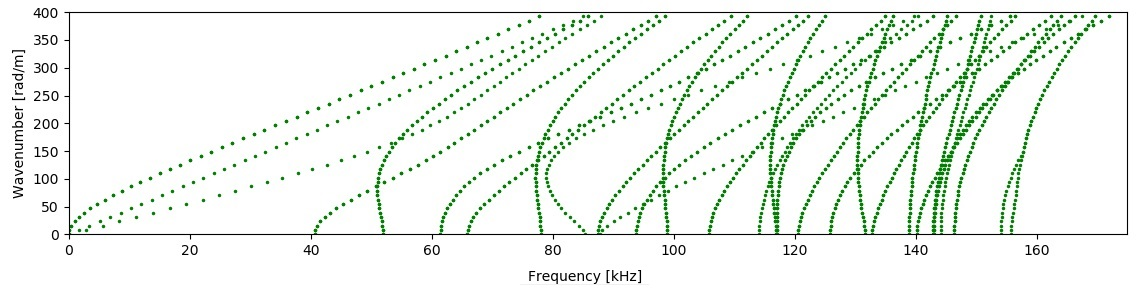
\includegraphics[width=14cm]{Zdjecia/2/przykladowe_krzywe}
\caption{Krzywe uzyskane przez wielokrotne rozwiązanie zagadnienia własnego pręta}
\label{fig:przykladowe_krzywe}
\end{figure}

